
C++标准库提供了一系列随机数分布生成器,每个生成器都有自己的属性。本节中,我们检查一个函数,通过创建输出的直方图来比较不同的选项。

\subsubsection{How to do it…}

与随机数引擎一样,分布生成器也有一些公共的接口元素。与随机数引擎不同,分布生成器有各种属性可以设置。可以创建一个模板函数来打印各种分布的直方图,但各种分布生成器的初始化差异很大:

\begin{itemize}
\item 
先从一些常数开始:

\begin{lstlisting}[style=styleCXX]
constexpr size_t n_samples{ 10 * 1000 };
constexpr size_t n_max{ 50 };
\end{lstlisting}

n\_samples常数是为每个直方图生成的样本数量——在本例中为10,000。

生成直方图时,n\_max常数作为除数。

\item 
直方图函数以分布生成器作为参数,并打印该分布算法的直方图:

\begin{lstlisting}[style=styleCXX]
void dist_histogram(auto distro,
		const string_view& dist_name) {
	std::default_random_engine rng{};
	map<long, size_t> m;
	
	// create the histogram map
	for(size_t i{}; i < n_samples; ++i)
		++m[(long)distro(rng)];
	
	// print the histogram
	auto max_elm_it = max_element(m.begin(), m.end(),
		[](const auto& a, const auto& b)
		{ return a.second < b.second; }
		);
	size_t max_elm = max_elm_it->second;
	size_t max_div = std::max(max_elm / n_max,
		size_t(1));
	cout << format("{}:\n", dist_name);
	for (const auto [randval, count] : m) {
		if (count < max_elm / n_max) continue;
		cout << format("{:3}:{:*<{}}\n",
			randval, ' ', count / max_div);
	}
}
\end{lstlisting}

dist\_histogram()函数的作用是:使用map来存储直方图。然后,在控制台上以星号的形式显示直方图。

\item 
在main()调用dist\_histogram():

\begin{lstlisting}[style=styleCXX]
int main() {
	dist_histogram(std::uniform_int_distribution<int>
		{0, 9}, uniform_int_distribution");
	dist_histogram(std::normal_distribution<double>
		{0.0, 2.0}, "normal_distribution");
	...
\end{lstlisting}

调用dist\_histogram()函数比调用随机数生成器要复杂得多。每个随机分布类别根据其算法有不同的参数集。

要获得完整的列表,请参考GitHub库中的distribution.cpp文件。

输出为:

\begin{center}
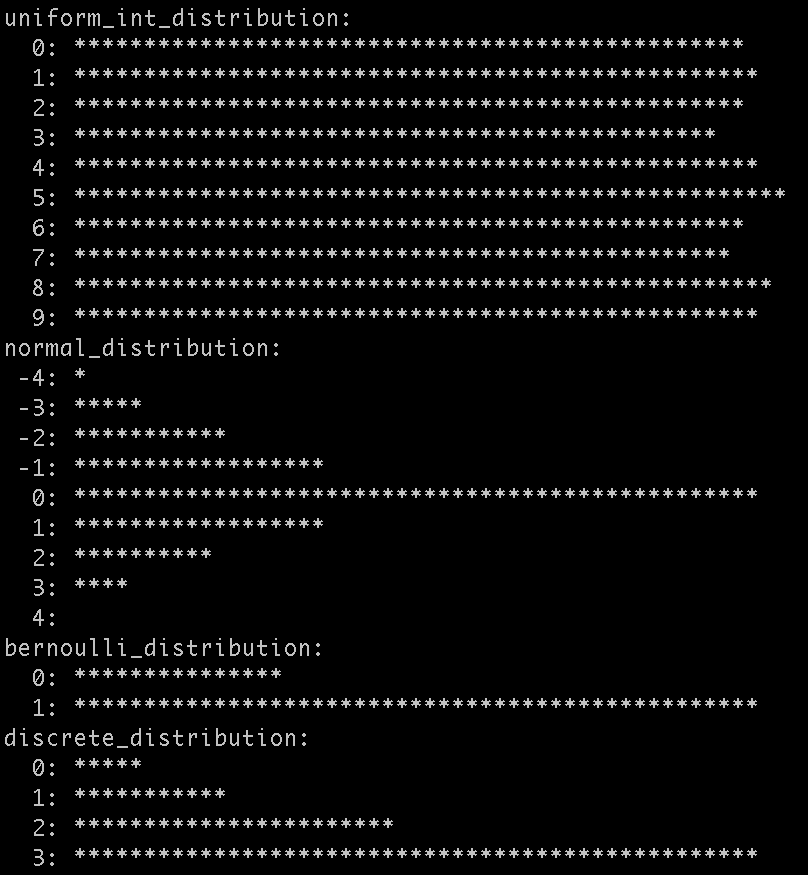
\includegraphics[width=0.6\textwidth]{content/chapter8/images/3.png}\\
图8.3 随机分布直方图的截图
\end{center}

每种分布算法产生非常不同的输出,可以试一下每个随机分布生成器的不同选项。

\end{itemize}

\subsubsection{How it works…}

每个分布生成器都有一个返回随机分布中下一个值的函子:

\begin{lstlisting}[style=styleCXX]
result_type operator()( Generator& g );
\end{lstlisting}

函子以随机数生成器(RNG)对象作为参数:

\begin{lstlisting}[style=styleCXX]
std::default_random_engine rng{};
map<long, size_t> m;
for (size_t i{}; i < n_samples; ++i) ++m[(long)distro(rng)];
\end{lstlisting}

现在,我们在RNG中使用std::default\_random\_engine。

与RNG直方图一样,这是一个有用的工具,可以可视化随机库中可用的各种随机分布算法。可以对每种算法可用的各种参数进行试验。











